\begin{center}
\textsc{\Large Laboratorio 7}~\\
{\large Vídeo Juegos, Programación, Diseño}~\\
\emph{Event Logging y Manejo de Usuarios}
\end{center}

\section{Pre-Laboratorio}
\todo[inline]{Por hacer.}

\section{Event Logging}
\setlength\intextsep{0pt}
\begin{wrapfigure}[11]{l}{0.3\linewidth}
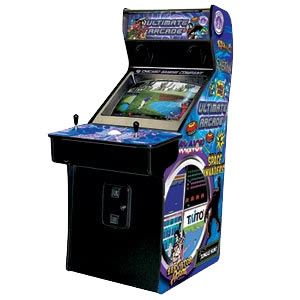
\includegraphics[width=\linewidth]{semana7/arcade-machines.jpg}
\caption{Los Arcade fueron los primeros vídeo juegos en considerar varios usuarios, guardando un pequeño ID y puntuación \cite{arcade_score}.}
\label{fig:arcade}
\end{wrapfigure}
Los vídeo juegos actuales son piezas de software de gran complejidad por lo tanto mantener un historial de información durante la ejecución del programa puede ser de inmensa ayuda para distintos propósitos. Esta información es usualmente utilizada para debugging pero dependiendo del tipo de información guardada esta puede ser usada para una gran cantidad de propósitos \cite{colm_tracing}.

\section{Manejo de Usuarios}
Los vídeo juegos usualmente puede ser jugados por mas de un usuario incluso si este vídeo juego es de un solo jugador, con cada usuario teniendo su propia sesión de juego, esta sesión de juego puede guardar cosas tan sencillas como el nombre de usuario para propósitos de personalización o datos mas complejos como actual posición en el transcurso del juego, puntuación, logros, objetivos actuales, etcétera, todo esto dependiente del diseño del juego.

\section{Actividad}
\todo[inline]{Por hacer.}